 \section{Multiple Host Ambiguities}
In parsing and interpreting the HTTP semantics,  one of the most important designations is what host is involved with the request, because \texttt{Host} is the key protocol field for resource locating, request routing, caching, etc. The problem of multiple host ambiguities arises when two parties (the downstream and upstream) in an HTTP processing-chain parse and interpret host in a crafted, adversarial request  differently. Inconsistency of host between two parties often causes disastrous consequences because of its semantic importance. 

\hspace{1 cm}--- \textit{Host of Troubles: Multiple Host Ambiguities in HTTP Implementations}

\subsection{Multiple Host Headers}
\label{sec:Multiple_Host_Headers}
RFC 2616\cite{rfc2616} states that a request with multiple same name headers is allowed only if the value of this header is defined as a single comma-separated list, which implies that a request with multiple \texttt{Host} headers is invalid.
RFC 7230 \cite{rfc7230} explicitly specifies that requests with multiple
\texttt{Host} headers must be reject with 400 Bad Request.

\hspace{1 cm}--- \textit{Host of Troubles: Multiple Host Ambiguities in HTTP Implementations}

\textbf{RFC 2616}
\columnseprule=1pt    %实现插入分隔线
\begin{multicols}{2}  %将该部分分两栏并在两栏列缝间插入分隔线
	\begin{spacing}{0.8} %将Specification中的部分设置为0.8倍行间距
		\textbf{4.2}
		{\footnotesize Multiple message-header fields with the same field-name MAY be present in a message if and only if the entire field-value for that header field is defined as a \textbf{comma-separated list}. It must be possible to combine the multiple header fields into one ``\texttt{field-name:field-value}" pair, without changing the semantics of the message, by appending each subsequent field-value to the first, each separated by a comma. The order in which header fields with the same field-name are received is therefore significant to the interpretation of the combined field value, and thus a proxy MUST NOT change the order of these field values when a message is forwarded. }
	
	\textbf{5.2} 
	{\footnotesize The exact resource identified by an Internet request is determined by \textbf{examining both the Request-\texttt{URI} and the \texttt{Host} header field}.\vspace{1ex}	
	%	An origin server that does not allow resources to differ by the requested host MAY ignore the Host header field value when determining the resource identified by an HTTP/1.1 request.
	An origin server that does differentiate resources based on the host requested (sometimes referred to as virtual hosts or vanity host names) MUST use the following rules for determining the requested resource on an HTTP/1.1 request:	
		\begin{enumerate}
			\item If Request-\texttt{URI} is an absolute\texttt{URI}, the host is part of the Request-\texttt{URI}. Any \texttt{Host} header field value in the request MUST be ignored.
			\item If the Request-\texttt{URI} is not an absolute\texttt{URI}, and the request includes a \texttt{Host} header field, the host is determined by the \texttt{Host} header field value.
			\item If the host as determined by rule 1 or 2 is not a valid host on the server, the response MUST be a 400 (Bad Request) error message.
		\end{enumerate}	
	Recipients of an HTTP/1.0 request that lacks a \texttt{Host} header field MAY attempt to use heuristics (e.g., examination of the URI path for something unique to a particular host) in order to determine what exact resource is being requested.}\vspace{1.2ex}
	\textbf{14.23}
	{\footnotesize A client MUST include a \texttt{Host} header field in all HTTP/1.1 request messages . If the requested \texttt{URI} does not include an Internet host name for the service being requested, then the \texttt{Host} header field MUST be given with an empty value. An HTTP/1.1 proxy MUST ensure that any request message it forwards does contain an appropriate \texttt{Host} header field that identifies the service being requested by the proxy. All Internet-based HTTP/1.1 servers MUST respond with a 400 (Bad Request) status code to any HTTP/1.1 request message which lacks a \texttt{Host} header field.}
	
	\textbf{19.6.1.1}
	{\footnotesize It is extremely important that all implementations of HTTP (including updates to existing HTTP/1.0 applications) correctly implement these requirements:
		\begin{itemize}
			\item Both clients and servers MUST support the \texttt{Host} request-header.
			\item A client that sends an HTTP/1.1 request MUST send a \texttt{Host} header.
			\item Servers MUST report a 400 (Bad Request) error if an HTTP/1.1
				request does not include a \texttt{Host} request-header.
			\item Servers MUST accept absolute \texttt{URIs}.
		\end{itemize}
		}
	\end{spacing}
\end{multicols}

\textbf{RFC 7230}
\columnseprule=1pt    %实现插入分隔线
\begin{multicols}{2}
	\begin{spacing}{0.8}
	\textbf{5.4}
	{\footnotesize A server MUST respond with a 400 (Bad Request) status code to any HTTP/1.1 request message that \textbf{lacks a Host header} field and to any request message that \textbf{contains more than one Host header} field or a Host header field with an \textbf{invalid field-value}.}
	\end{spacing}
\end{multicols}

\subsection{Space-surrounded Host Header}
\subsubsection{The first header with preceding space}
RFC 2616 does not have explicit text for this case. The syntax definition implies that systems should reject the request with a space preceding the first header. RFC 7230 suggests to either reject the request or ignore the header.

\textbf{RFC 2616}
\columnseprule=1pt    %实现插入分隔线
\begin{multicols}{2}
	\begin{spacing}{0.8}
		\textbf{} 
		{\footnotesize  }
	\end{spacing}
\end{multicols}

\textbf{RFC 7230}
\columnseprule=1pt    %实现插入分隔线
\begin{multicols}{2}
	\begin{spacing}{0.8}
		\textbf{3.} 
		%关于前带空格的header的处理
		{\footnotesize 
		A sender MUST NOT send whitespace between the start-line and the
		first header field. \textbf{A recipient that receives whitespace between the start-line and the first header field MUST either reject the message} as invalid or consume each whitespace-preceded line without further processing of it (i.e., \textbf{ignore the entire line}, along with any subsequent lines preceded by whitespace, until a properly formed header field is received or the header section is terminated).\vspace{1ex} \\ 
		The presence of such whitespace in a request might be an attempt to trick a server into ignoring that field or processing the line after it as a new request, either of which might result in a security vulnerability if other implementations within the request chain interpret the same message differently.\\	
		}
		\textbf{3.2.4} 
	    {\footnotesize  The field value does not include any leading or trailing whitespace: \textbf{OWS occurring before the first non-whitespace octet of the field value} or after the last non-whitespace octet of the field value \textbf{ought to be excluded} by parsers when extracting the field value from a header field.}
	\end{spacing}
\end{multicols}

\subsubsection{Non-first header with preceding space}
RFC 2616 states that a such header needs to be processed as folded line of its previous header: remove its preceding line break characters to concatenate with the
previous header. Although RFC 7230 already obsoletes line folding, it still allows a proxy or a server to process as line folding for backward compatibility considerations.

\hspace{1 cm}--- \textit{Host of Troubles: Multiple Host Ambiguities in HTTP Implementations}

\textbf{RFC 2616}
\columnseprule=1pt    %实现插入分隔线
\begin{multicols}{2}
	\begin{spacing}{0.8}
		\textbf{2.2} 
		{\footnotesize  \textbf{HTTP/1.1 header field values can be folded onto multiple lines if the continuation line begins with a space or horizontal tab.} All linear white space, including folding, has the same semantics as SP. A recipient MAY replace any linear white space with a single SP before interpreting the field value or forwarding the message downstream. }
	\end{spacing}
\end{multicols}

\textbf{RFC 7230}
\columnseprule=1pt    %实现插入分隔线
\begin{multicols}{2}
	\begin{spacing}{0.8}
		\textbf{3.2.4} 
		{\footnotesize Historically, HTTP header field values could be extended over
		multiple lines by preceding each extra line with at least one space or horizontal tab (obs-fold).\textbf{ This specification deprecates such line folding except within the message/http media type.}}
	\end{spacing}
\end{multicols}

\subsubsection{Headers with succeeding space}
RFC 2616 does not have explicit text for this case. The syntax definition implies that systems should allow this request. The same situation is explicitly forbidden in RFC 7230.

\textbf{RFC 2616}
\columnseprule=1pt    %实现插入分隔线
\begin{multicols}{2}
	\begin{spacing}{0.8}
		\textbf{} 
		{\footnotesize  }
	\end{spacing}
\end{multicols}

\textbf{RFC 7230}
\columnseprule=1pt    %实现插入分隔线
\begin{multicols}{2}
	\begin{spacing}{0.8}
		\textbf{3.2.4} 
		{\footnotesize  A field value might be preceded and/or followed by optional
			whitespace (OWS). The field value does not include any leading or trailin whitespace: \textbf{OWS occurring} before the first non-whitespace octet of the field value or \textbf{after the last non-whitespace octet of the field value ought to be excluded} by parsers when extracting the field value from a header field.}
	\end{spacing}
\end{multicols}

\begin{figure*}[!htbp]
	\centering
	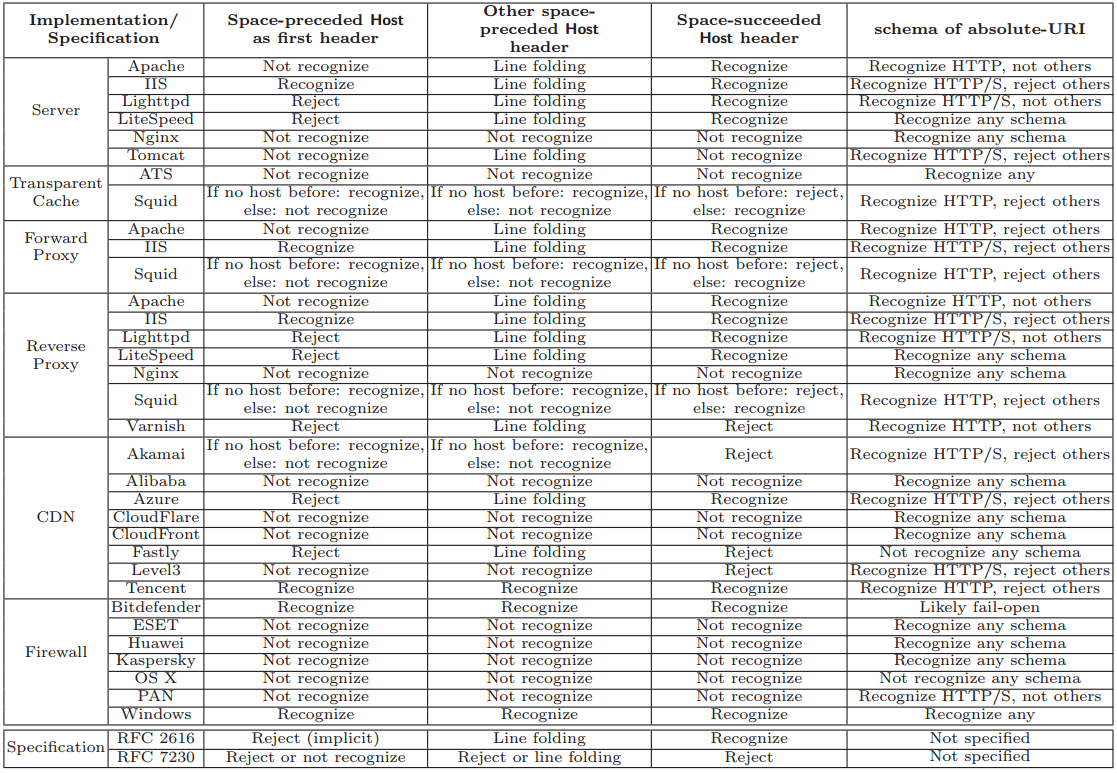
\includegraphics[width=1.0\textwidth]{Host_Parsing.jpg}
	\caption{Host parsing behaviors. Specifications and tested implementations (``recognize" means accepting as valid host field, ``not recognize" means either ignoring or accepting as an unknown header field, ``reject" means responding with 400 Bad Request).}
	\label{fig:host_parsing}
\end{figure*}
\subsection{Absolute-URI as Request-Target}
Both RFC 2616 and RFC 7230 require server to accept absolute-\texttt{URI} as request-target, and to prefer host component of absolute-\texttt{URI} than \texttt{Host} header. RFC 7230 additionally requires requests with absolute-URI to have identical host component as \texttt{Host} header. Both of the two RFCs do not explicitly state which schema is allowed in the absolute-URI.

\textbf{RFC 2616}
\columnseprule=1pt    %实现插入分隔线
\begin{multicols}{2}
	\begin{spacing}{0.8}
		\textbf{5.2} 
		{\footnotesize See the ``RFC 2616" part in section \ref{sec:Multiple_Host_Headers}.}
	\end{spacing}
\end{multicols}

\textbf{RFC 7230}
\columnseprule=1pt    %实现插入分隔线
\begin{multicols}{2}
	\begin{spacing}{0.8}
		\textbf{5.5} 
		{\footnotesize 
		\textbf{Since the request-target often contains only part of the user agent’s target URI, a server reconstructs the intended target as an ``effective request URI" to properly service the request}. This reconstruction involves both the \textbf{server’s local configuration} and information communicated in the \textbf{request-target}, \textbf{\texttt{Host} header field}, and \textbf{connection context}.\vspace{1.2ex}\\
		For a user agent, the effective request URI is the target URI. If the request-target is in absolute-form, the effective request URI is the same as the request-target. Otherwise, the effective request URI is constructed as follows:
	
		\begin{enumerate}
			\item If the server’s configuration (or outbound gateway) provides a
			fixed URI \textbf{scheme}, that scheme is used for the effective request URI. Otherwise, if the request is received over a TLS-secured TCP connection, the effective request URI’s scheme is "https"; if not, the scheme is "http".
			\item If the server’s configuration (or outbound gateway) provides a fixed URI \textbf{authority component}, that authority is used for the effective request URI. If not, then if the request-target is in authority-form, the effective request URI’s authority component is the same as request-target. If not, then if a \texttt{Host} header field is supplied with a non-empty field-value, the authority component is the same as the \texttt{Host} field-value. Otherwise, the authority component is assigned the default name configured for the server and, if the connection’s incoming TCP port number differs from the default port for the effective request URI’s scheme, then a colon (":") and the incoming port number are appended to the authority component.
			\item If the request-target is in authority-form or asterisk-form, the
			effective request URI’s combined path and query component is empty. Otherwise, the combined path and query component is the same as the request-target.
		
		\end{enumerate}
	
		The components of the effective request URI, once determined as above, can be combined into absolute-URI form by concatenating the \textbf{scheme}, "://", \textbf{authority}, and \textbf{combined path and query component}. }
	\end{spacing}
\end{multicols}	
	



